\begin{comment}
\end{comment}

\chapter{Comptage variationnel quantique}

%-----------------------------------------------------------------------------%

\begin{comment}
\subsection*{Plan}

\begin{enumerate}
    \item Expliquer que cette section ne concerne que GM-QAOA
\end{enumerate}
\end{comment}

L'apport principal de ce travail réside dans la combinaison des algorithmes variationnels quantique avec l'algorithme de JVV.



d'échantillonner la distribution préparée par un algorithme variationnel quantique afin de produire un compte approximatif à l'aide de l'algorithme de JVV. 

\textcolor{mydarkred}{\textit{Parler de pourquoi QAOA ne peut pas résoudre efficacement les problèmes de comptage.}}



%-----------------------------------------------------------------------------%

\section{Algorithme VQCount}

\begin{comment}
\subsection*{Plan}

\begin{enumerate}
    \item Vulgariser l'algorithme de manière général
    \item Expliquer rigoureusement l'algorithme
    \item Faire le lien entre la notation utilisée dans les algorithmes de comptage classique
    \item Faire la comparaison avec les travaux précédents
    \item Rajouter l'algorithme complet en pseudo-code
\end{enumerate}

\subsection*{Références}
\end{comment}

Comment faire le pont entre les algorithmes variationnels quantiques et l'algorithme de JVV pour la résolution de problème de comptage? À priori, l'algorithme de JVV doit tout simplement être implémenté en utilisant un algorithme variationnel quantique comme générateur de solutions. Cependant, plusieurs embûches barrent notre chemin. Décrivons la procédure, nommé VQCount par brièveté, en affrontant ces problèmes en chemin.

Soit une instance de problème SAT, décrite par la formule CNF $\varphi$. Ce problème est auto-réductible par la relation~\ref{rel:auto-reductibilite-sat}. Ce travail se limite à l'étude du problème SAT en gardant en tête que par sa \textsf{NP}-complétude, une réduction existe entre n'importe quel problème de la classe \textsf{NP} et celui-ci. \textcolor{mydarkred}{\textit{Potentiellement d'autres problèmes avec }}. La formule $\varphi$ peut être transformée en un modèle d'Ising, tel que décrit à la section~\ref{subsec:encodage-probleme}, dont l'Hamiltonien $H_{P}$ encode le problème. Grâce à cet Hamiltonien de problème, il est possible de construire le circuit paramétré quantique de l'algorithme QAOA, préparant l'état $\ket{\psi(\vec{\gamma_{0}}, \vec{\beta_{0}})}$. Négligeons pour le moment le choix de l'état initial et de l'Hamiltonien de forçage. Une fois le circuit construit, l'énergie moyenne de $H_{P}$ est évalué en mesurant l'état préparé. Un optimiseur classique modifie alors les paramètres du circuit quantique pour minimiser cette énergie, donnant un circuit quantique paramétré optimisé $\ket{\psi(\vec{\gamma}, \vec{\beta})}$.
Les échantillons, obtenus par une mesure dans la base computationnelle de l'état préparé par le circuit, contient alors, avec une haute probabilité, des solutions à la formule $\varphi$.

\textcolor{mydarkred}{\textit{Peut-être raccourcir?}}

Comme QAOA est une heuristique, les paramètres optimaux ne sont pas nécessairement atteints, impliquant la présence de non-solutions dans la distribution obtenue en mesurant $\ket{\psi(\vec{\gamma}, \vec{\beta})}$. Comme l'algorithme de JVV nécessite une distribution composée uniquement de solutions, une étape de post-traitement doit être employé pour retirer les non-solutions. Comme le problème SAT appartient à la classe \textsf{NP}, vérifier qu'un échantillon est une solution est un processus efficace. Ainsi, toutes les non-solutions échantillonnées sont retirés de la distribution obtenue. De plus, comme discuté à la section~\ref{sec:echantillonage-et-biais}, la non-uniformité de la distribution obtenue ne respecte pas nécessairement la condition de l'algorithme de JVV. La discussion dans cette section se restreindra alors à la variante GM-QAOA, qui garantie que l'amplitude des solutions de $\ket{\psi(\vec{\gamma}, \vec{\beta})}$ soit égale. 

Ces remarques complétées, $O(\frac{n \log (\delta)}{r \varepsilon^{2}})$ échantillons sont mesurées du circuit. En utilisant ces échantillons, la valeur la plus probable de la première variable $w_{0}$ à est déterminée. Selon l'algorithme de JVV, il faut alors résoudre le sous-instance $\varphi_{w_{0}}$. Résoudre directement celle-ci à l'aide du même circuit optimisé demanderait une post-sélection supplémentaire sur la première variable. En réalité, comme il existe un nombre exponentiel de sous-instances, en raison du nombre exponentiel de chaîne de bit possible, il faudrait retirer un nombre exponentiel d'échantillons supplémentaires. Une autre méthode consisterait à construire et optimiser un différent circuit pour résoudre la sous-instance. Pour éviter tout cela, le circuit de GM-QAOA est modifié pour chaque sous-problème tel qu'illustré à la figure~\ref{fig:quantum-circuit}. Cette modification permet de conserver la propriété d'égalité des amplitudes de GM-QAOA tout en suggérant qu'il est possible de garder les mêmes paramètres. \textcolor{mydarkred}{\textit{Compléter.}}

Le processus précédent est ensuite répété, jusqu'à ce que toutes les variables sont fixées. Le nombre de solutions est alors données par l'inverse du produit des probabilités conditionnelles.

D'abord, le problème de comptage est encodé dans un circuit quantique selon l'algorithme QAOA. 




Suite à l'optimisation de ce circuit par un optimiseur classique, une distribution de solutions est obtenue. De cette distribution, plusieurs solutions sont échantillonnées. Finalement, QAOA est à nouveau utilisé comme générateur pour les sous-problèmes de manière récursive.




Quelques remarques sont nécessaires avant d'expliquer en profondeur l'algorithme VQCount. Rappelons d'abord les conditions nécessaires à l'algorithme de comptage approximatif.

\begin{enumerate}[(1)]
    \item \textbf{Auto-réductibilité:} Le problème de comptage doit être auto-réductible.
    \item \textbf{Générateur de solutions:} Le générateur de solutions doit être en mesure de retourner des solutions pour toutes les sous-instances du problème.
    \item \textbf{Nonuniformité:} Le générateur de solutions doit être quasi uniforme, c'est-à-dire dont la distribution de solutions tend vers l'inverse du nombre de variables.
\end{enumerate}

Pour la première contrainte, ce travail se limite à l'étude du problème SAT, auto-réductible par la relation~\ref{rel:auto-reductibilite-sat}. Celui-ci étant \textsf{NP}-complet, une réduction existe alors pour tout problème de la classe \textsf{NP}. \textsf{Autre problème avec transformation d'Ising?}. 

Pour la deuxième contrainte, 





L'algorithme VQCount utilise l'état préparé par un circuit GM-QAOA comme générateur de solutions pour obtenir un compte approximatif en se basant sur l'algorithme de JVV. 

Comment est-ce que l'algorithme VQCount opère? Soit un problème SAT, décrit par une formule CNF $\varphi(x)$. Ce problème   




\begin{algorithm}[b!]
    \caption{VQCount}\label{alg:vqcount}
    \begin{algorithmic}[1]
    \REQUIRE CNF formula: $f(n, m)$, Problem: $P$,  Depth: $p$, Minimum energy: $E_{min}$, Accuracy: $\varepsilon$, Confidence: $\delta$, Optimizer: $O$, Optimization tolerance: $\varepsilon_{opt}$, Maximum number of optimization steps: $n_{opt}^{max}$
    
    \STATE $H_P \leftarrow$ Mapping($f(n, m)$, $P$)
    \STATE $H_D \leftarrow$ Grover-Mixer(n)
    \STATE $i$, $j$ $\leftarrow$ $0$
    \STATE $x, r, N \leftarrow [0]^n$
    \STATE $\Tilde{p} \leftarrow [0]^{n+1}$
    \FOR{$k \textbf{ in } 1 \textbf{ to } 2\log_{\frac{3}{4}}(\frac{1}{\delta})+1$}
    \WHILE{$i < n$ \textbf{and} $\Tilde{p}(i) < 1$}
    \STATE $\gamma$, $\beta$ $\leftarrow$ TQA($H_P$, $H_D$, $p$)
    \STATE PQC($\gamma$, $\beta$)  $\leftarrow$ VQCount-QAOA($H_P$, $H_D$, $\gamma$, $\beta$, $p$, $x$)
    \STATE $E$ $\leftarrow$ Energy(PQC($\gamma$, $\beta$))
    \WHILE{$E > E_{min} (1+\text{sgn}(E_{min})\varepsilon_{opt}) \textbf{ and } j \leq n_{opt}^{max}(i)$}
    \STATE $\text{PQC}(\gamma, \beta) \leftarrow \text{Optimizer}(\text{PQC}(\gamma, \beta), opt)$
    \STATE $j \leftarrow j + 1$
    \ENDWHILE
    \STATE $s \leftarrow \text{Solution-Sampler}(\text{PQC}(\gamma, \beta), n^3)$
    \STATE $x(i), \Tilde{p}(i+1) \leftarrow \text{Prob}(s)$
    \STATE $i \leftarrow i + 1$
    \ENDWHILE
    \STATE $ \Tilde{p}^* \leftarrow \prod_{q = 0}^{n-1}\Tilde{p}(q)$
    \STATE $N(i) \leftarrow \frac{1}{\Tilde{p}^*}$
    \ENDFOR
    \STATE $N^* \leftarrow \text{Median}(N)$
    \STATE Return $N^*$
    \end{algorithmic}
\end{algorithm}
    


%-----------------------------------------------------------------------------%

\section{Auto-réductibilité des algorithmes variationnels quantiques}

\subsection*{Plan}

\begin{enumerate}
    \item Faire la preuve de l'auto-réductibilité des algorithmes variationnels quantiques
\end{enumerate}

\subsection*{Références}

% \begin{figure}[t]
%     \centering
%     \begin{quantikz}[font=\sffamily]
%       \ket{0} & \gate[style={fill=mysilver!80}][0.80cm]{H} & \gate[wires=4, nwires=3, style={fill=myblue}][1.30cm]{U_P (\gamma_{1})} & \gate[wires=4, nwires=3, style={fill=myred}][1.30cm]{U_D (\beta_{1})} & \ \ldots\ \qw & \gate[wires=4, nwires=3, style={fill=myblue}][1.30cm]{U_P (\gamma_{p})} & \gate[wires=4, nwires=3, style={fill=myred}][1.30cm]{U_D (\beta_{p})} & \qw \\
%       \ket{0} & \gate[style={fill=mysilver!80}][0.80cm]{H} & & & \ \ldots\ \qw & & & \qw \\
%       \vdots & & & & & & & \\
%       \ket{0} & \gate[style={fill=mysilver!80}][0.80cm]{H} & & & \ \ldots\ \qw & & & \qw
%     \end{quantikz}
%     \caption{}
% \end{figure}

% \begin{figure}[t]
%     \centering
%     \begin{quantikz}
%       \ket{0} & \gate[style={fill=myyellow!80}][0.80cm]{X^{c}} & \gate[wires=4, nwires=3, style={fill=myblue}][1.30cm]{U_P (\gamma_{1})} & \qw & \ \ldots\ \qw & \gate[wires=4, nwires=3, style={fill=myblue}][1.30cm]{U_P (\gamma_{p}) } & \qw & \qw \\
%       \ket{0} & \gate[style={fill=mysilver!80}][0.80cm]{H} & & \gate[wires=3, nwires=2, style={fill=myred}][1.30cm]{U_D (\beta_{1})} & \ \ldots\ \qw & & \gate[wires=3, nwires=2, style={fill=myred}][1.30cm]{U_D (\beta_{p})} & \qw \\
%       \vdots & & & & & & & \\
%       \ket{0} & \gate[style={fill=mysilver!80}][0.80cm]{H} & & & \ \ldots\ \qw & & & \qw
%     \end{quantikz}
%     \caption{}
% \end{figure}

% \begin{figure}[h]
%     \centering
%     \begin{quantikz}
%         \ket{x_1} & \ctrl{3} & \qw      & \qw      & \qw      & \qw      & \qw      & \qw      & \qw      & \qw      & \qw      & \qw      & \qw     & \ctrl{3} & \qw \\
%         \ket{x_2} & \qw      & \ctrl{2} & \ctrl{3} & \qw      & \qw      & \qw      & \qw      & \qw      & \qw      & \qw      & \ctrl{3} & \ctrl{2}     & \qw      & \qw \\
%         \ket{x_3} & \qw      & \qw      & \qw      & \ctrl{2} & \qw      & \qw      & \qw      & \qw      & \qw      & \ctrl{2} & \qw      & \qw     & \qw      & \qw \\
%         \ket{0}   & \targ{}  & \targ{}  & \qw      & \qw      & \targ{}  & \ctrl{2}      & \qw      & \ctrl{2} & \targ{}  & \qw      & \qw      & \targ{}      & \targ{}  & \qw \\
%         \ket{0}   & \qw      & \qw      & \targ{}  & \targ{}  & \targ{}  & \ctrl{1}      & \qw     & \ctrl{1}  & \targ{}  & \targ{}  & \targ{}  & \qw     & \qw     & \qw \\
%         \ket{0}   & \qw      & \qw      & \qw      & \qw      & \qw      & \targ{}       & \ctrl{7} & \targ{}  & \qw      & \qw      & \qw      & \qw     & \qw      & \qw \\ [0.5cm]
%         \ket{x_4} & \ctrl{3} & \qw      & \qw      & \qw      & \qw      & \qw      & \qw      & \qw      & \qw      & \qw      & \qw      & \qw     & \ctrl{3} & \qw \\
%         \ket{x_5} & \qw      & \ctrl{2} & \ctrl{3} & \qw      & \qw      & \qw      & \qw      & \qw      & \qw      & \qw      & \ctrl{3} & \ctrl{2}     & \qw      & \qw \\
%         \ket{x_6} & \qw      & \qw      & \qw      & \ctrl{2} & \qw      & \qw      & \qw      & \qw      & \qw      & \ctrl{2} & \qw      & \qw     & \qw      & \qw \\
%         \ket{0}   & \targ{}  & \targ{}  & \qw      & \qw      & \targ{}  & \ctrl{2}      & \qw      & \ctrl{2} & \targ{}  & \qw      & \qw      & \targ{}      & \targ{}  & \qw \\
%         \ket{0}   & \qw      & \qw      & \targ{}  & \targ{}  & \targ{}  & \ctrl{1}      & \qw     & \ctrl{1}  & \targ{}  & \targ{}  & \targ{}  & \qw     & \qw     & \qw \\
%         \ket{0}   & \qw      & \qw      & \qw      & \qw      & \qw      & \targ{}       & \ctrl{1} & \targ{}  & \qw      & \qw      & \qw      & \qw     & \qw      & \qw \\ [0.5cm]
%         \ket{0}   & \qw      & \qw      & \qw      & \qw      & \qw      & \qw      & \gate{Z^{- \gamma \varepsilon/\pi}}  & \qw & \qw & \qw & \qw & \qw & \meter{} & \qw \\
%         \end{quantikz}
%     \caption{}
%     \label{fig:..}
% \end{figure}

\begin{figure*}[t]
    \centering
    \begin{subfigure}[h]{0.45\textwidth}
    \centering
    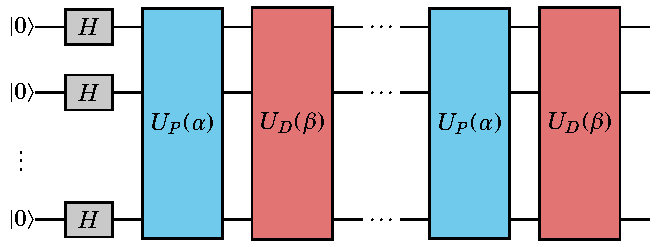
\includegraphics[width=1\textwidth]{figures/qaoa-self-reducibility-1.pdf}
    \caption{}
    \label{fig:quantum-circuit-a}
    \end{subfigure}
    \begin{subfigure}[h]{0.45\textwidth}
    \centering
    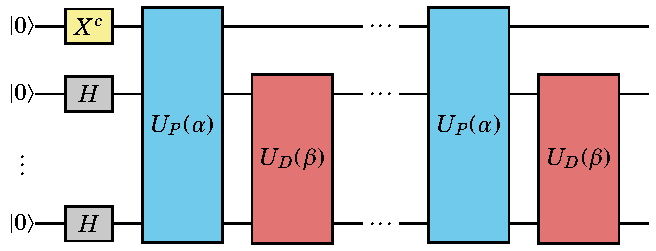
\includegraphics[width=1\textwidth]{figures/qaoa-self-reducibility-2.pdf}
    \caption{}
    \label{fig:quantum-circuit-b}
    \end{subfigure}
\caption{}
\label{fig:quantum-circuit}
\end{figure*}

% \begin{figure*}[h]
%     \centering
%     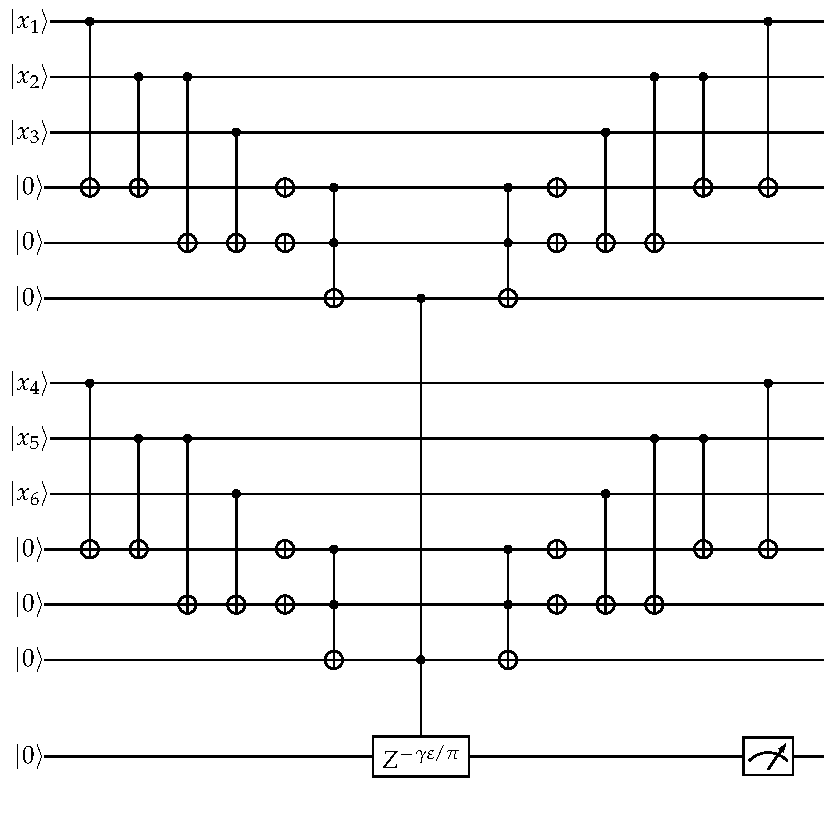
\includegraphics[width=0.6\textwidth]{figures/two-level-map.pdf}
%     \caption{}
%     \label{fig:two-level-map}
% \end{figure*}

%-----------------------------------------------------------------------------%

\section{Module VQCount}

\subsection*{Plan}

\begin{enumerate}
    \item Expliquer les librairies python dévelopées
    \item Décrire \textit{qaoa-quimb}
    \item Décrire \textit{VQCount}
\end{enumerate}

\subsection*{Références}